\documentclass{article}

% Environment setup

\usepackage[
    margin=1in
]{geometry} %geometry (sets margin) and other useful packages 
\setlength{\oddsidemargin}{.25in}
\setlength{\evensidemargin}{.25in}
\setlength{\textwidth}{6in}
\setlength{\topmargin}{-0.4in}
\setlength{\textheight}{8.5in}
\setlength{\parindent}{0em}
\setlength{\parskip}{.75em}

\usepackage{graphicx}
\usepackage{grffile}  % support extra dots in filenames
\usepackage{fancyref}
\usepackage[labelfont=bf]{caption}
\usepackage{subcaption}


\title{\textbf{CS 4641:} Randomized Optimization}
\author{Bradley Reardon}
\date{March 3, 2019}

\begin{document}
  \maketitle

  \section{Introduction}
  The purpose of this assignment is to evaluate various random search algorithms. Namely, the algorithms of interest that will be explored in this report are: randomized hill climbing, simulated annealing, genetic algorithms, and MIMIC.

  The first part of this report will focus on using the breast cancer dataset that was used for the previous assignment regarding supervised learning, along with the various search algorithms being used to optimize the weights for a neural network.

  The second part of the report will focus on distinguishing the strengths of each algorithm by applying each in the context of various optimization problems. \textbf{TODO optimization problems} 

  \subsection{Breast Cancer Wisconsin data set}
  The Breast Cancer Wisconsin data set was donated to the UCI Machine Learning Repository in 1992, and contains data from one doctor's clinical cases, gathered from January 1989 to November 1991. In total, there are 699 instances signifying information about breast tumors such as clump thickness, uniformity in shape and size, and other screening factors. Data points are identified by two classes -- benign or malignant. The features of the data points are encoded as 9 continuous attributes rating the screening factor from 1 to 10.

  This data set contains unknowns in the form of question marks in the data. Due to the nature of the implementations in ABAGAIL, these 16 data points containing unknowns were stripped from the data set. Therefore, the set used for this report contains 683 instances.

  The problem at hand for this data set is determining whether a tumor is benign or malignant based on tumor screening characteristics identified in the data set.

  \textbf{Source:} https://archive.ics.uci.edu/ml/datasets/Breast+Cancer+Wisconsin+\%28Original\%29

  \section{Optimizing Neural Network Weights}

  \subsection{Random Hill Climbing}

  \Fref{fig:rhc-params} shows the training and test error curves for the cancer data sets using randomized hill climbing for weight optimization. Each bar represents the training and test error at iteration \#1000 for varying numbers of restarts.

  \begin{figure}[htb]
  \centering

  \begin{subfigure}{0.5\textwidth}
    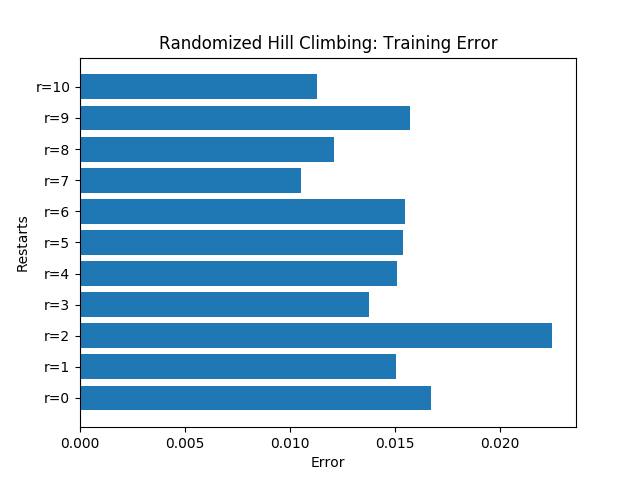
\includegraphics[width=\linewidth]{out/rhc/restarts-training.png}
    \caption{Training error}
    \label{fig:rhc-params-1}
  \end{subfigure}\hfil
  \begin{subfigure}{0.5\textwidth}
    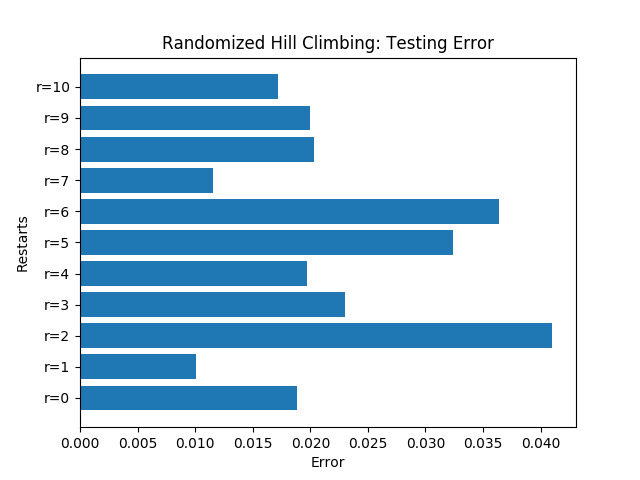
\includegraphics[width=\linewidth]{out/rhc/restarts-testing.png}
    \caption{Testing error}
    \label{fig:rhc-params-2}
  \end{subfigure}

  \caption{Learning curves for randomized hill climbing with varying restarts.}
  \label{fig:rhc-params}
  \end{figure}

  TODO TODO

  \Fref{fig:rhc-learning} shows the learning curves for the cancer data set, using randomized hill climbing with no restarts.

  \begin{figure}[htb]
  \centering
  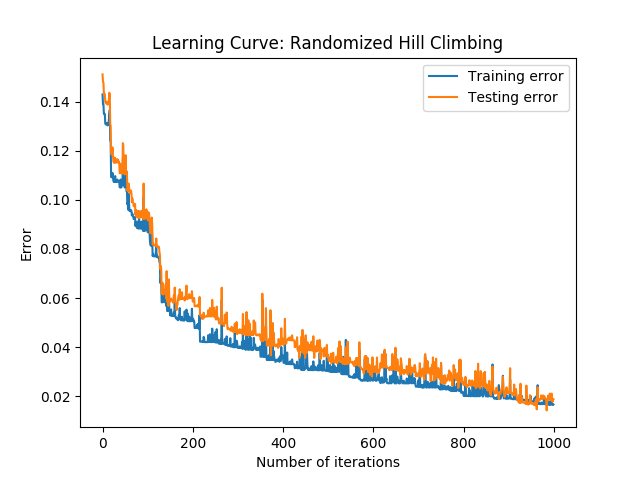
\includegraphics[width=.5\linewidth]{out/plot/RHC.png}
  \caption{Learning curve for random hill climbing.}
  \label{fig:rhc-learning}
  \end{figure}

  \subsection{Simulated Annealing}

  \Fref{fig:sa-params} shows the training and test error curves for the cancer data set using simulated annealing for weight optimization. The different series in the figure represent different cooling rates.

  \begin{figure}[htb]
  \centering

  \begin{subfigure}{0.5\textwidth}
    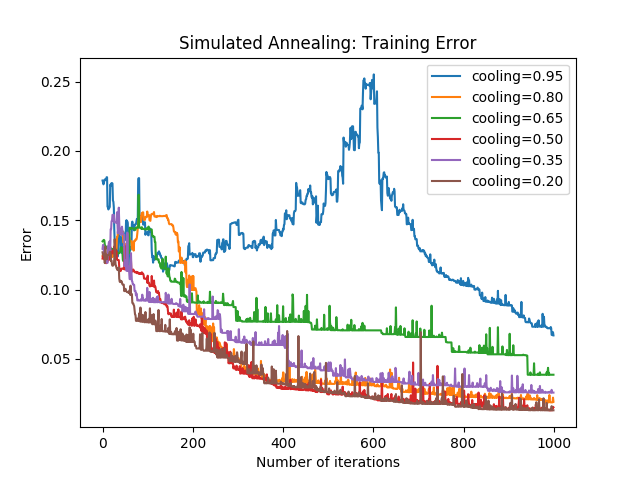
\includegraphics[width=\linewidth]{out/sa/cooling-error-training.png}
    \caption{Training error}
    \label{fig:sa-params-1}
  \end{subfigure}\hfil
  \begin{subfigure}{0.5\textwidth}
    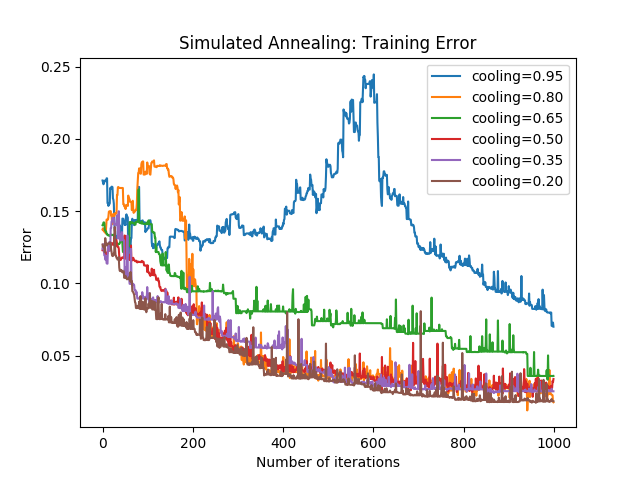
\includegraphics[width=\linewidth]{out/sa/cooling-error-testing.png}
    \caption{Testing error}
    \label{fig:sa-params-2}
  \end{subfigure}

  \caption{Learning curves for simulated annealing with different cooling rates.}
  \label{fig:sa-params}
  \end{figure}

  TODO TODO

  \Fref{fig:sa-learning} shows the learning curves for the cancer data set using simulated annealing.

  \begin{figure}[htb]
  \centering
  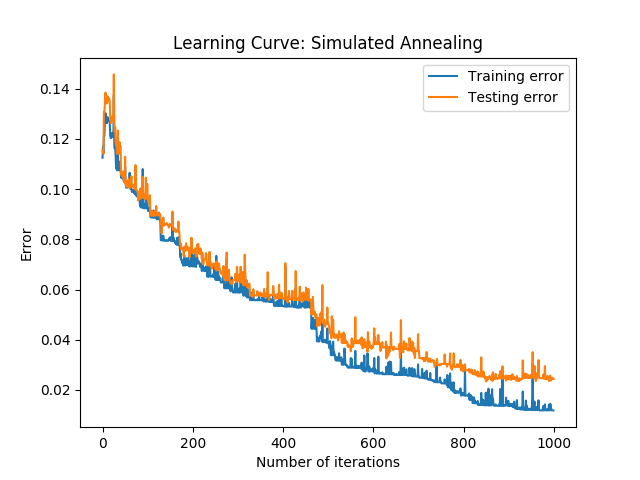
\includegraphics[width=.5\linewidth]{out/plot/SA.png}
  \caption{Learning curve for simulated annealing.}
  \label{fig:sa-learning}
  \end{figure}

  \subsection{Genetic Algorithms}

  \Fref{fig:ga-learning} shows the learning curves for the cancer data set using genetic algorithms.

  \begin{figure}[htb]
  \centering
  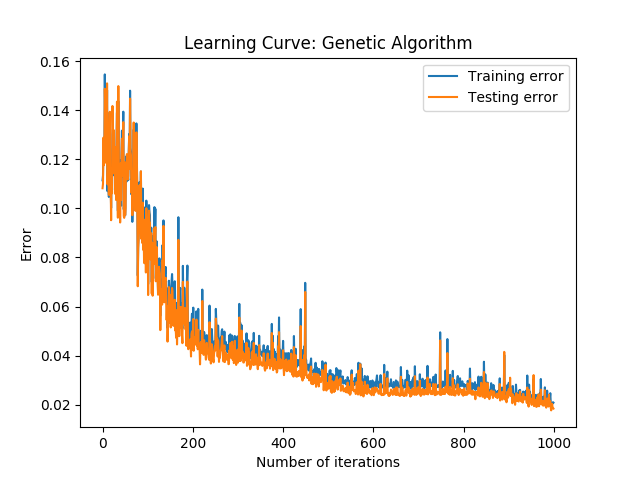
\includegraphics[width=.5\linewidth]{out/plot/GA.png}
  \caption{Learning curve for genetic algorithms.}
  \label{fig:ga-learning}
  \end{figure}

  \subsection{Comparison}

  \section{Exploring Optimization Problems}

  Blah blah here are the ones I chose

  \subsection{Simulated Annealing}
  Here's a problem good with SA

  \subsection{Genetic Algorithms}
  Here's a problem good with GA

  \subsection{MIMIC}
  Here's a problem good with MIMIC

  \section{Discussion}

  \section{Conclusion}



\end{document}